\subsection{Antagonism}\label{antagonism}

A fundamental principle in the body plan of bilaterians is the organization of movement through antagonistic pairs of effectors. Muscles, by their biological constitution, can only contract (i.e., pull) but not push. This morphological constraint necessitates the evolution of opposing pairs of muscles—flexors and extensors, abductors and adductors, pronators and supinators—that can act in reciprocal fashion to enable controlled motion \cite{Huxley1932_RelativeGrowth,Schilling2011_AntagonisticEvolution}. The bilaterian body plan, with its segmentation and bilateral symmetry, provides the structural basis for this arrangement.

At the neural level, antagonism is implemented by the canonical circuit motif of reciprocal inhibition. Sherrington’s classic work established that the activation of one muscle in a pair is accompanied by inhibition of its antagonist, ensuring coordinated and efficient movement \cite{Sherrington1906_IntegrativeAction}. This basic inhibitory scheme remains central to vertebrate and invertebrate motor control and underlies the formation of stable motor patterns.

From a biomechanical perspective, antagonistic control confers several advantages. Co-activation of antagonists allows modulation of joint stiffness, enabling both stability and compliance. Such mechanisms are critical for adaptive interaction with the environment and have inspired numerous robotic implementations of antagonistic actuators \cite{Hogan1984_ImpedanceControl,Tondu2012_McKibbenMuscle}. In biological systems, this provides the capacity not only to move but also to regulate impedance and precision.

In the context of the sensation-modulating network (SMN), antagonism is not merely a mechanical solution but also a higher-order organizational principle. Antagonistic structures encode dynamic balances: approach versus avoidance, activation versus inhibition, flexion versus extension. These embodied oppositions structure the repertoire of available action schemas and affordances, contributing to the cognitive architecture of the SMN itself \cite{Bizzi2013_MuscleSynergies}. Thus, antagonism serves as both a morphological constraint and a generative principle for embodied cognition.

\begin{figure}[htbp]
  \centering
  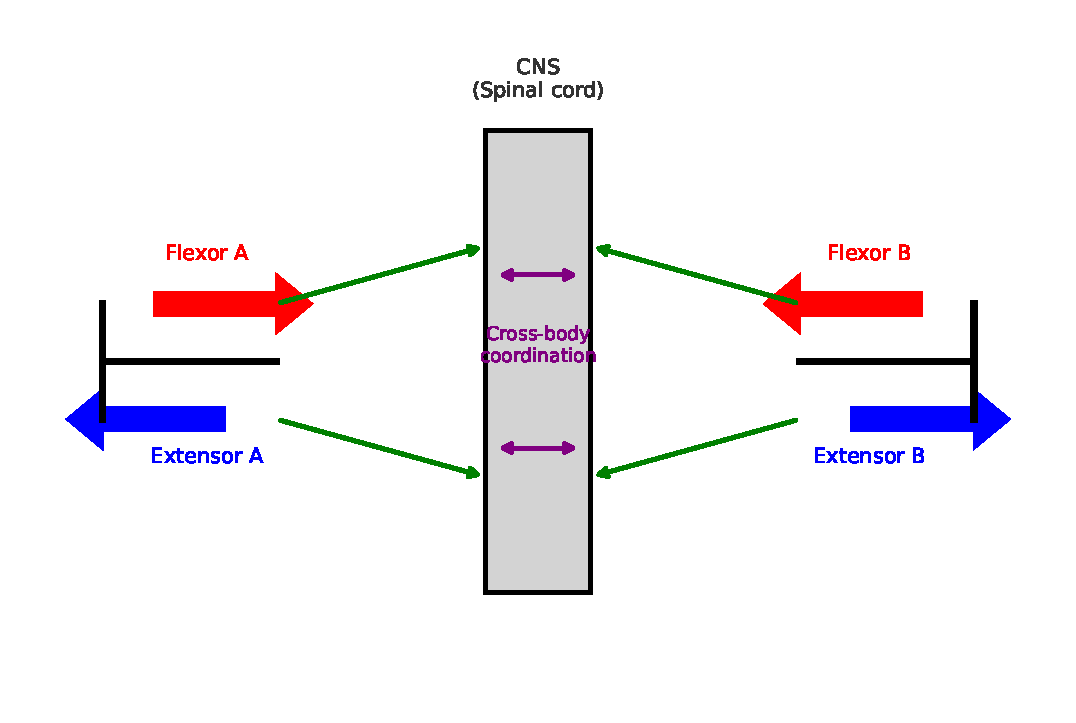
\includegraphics[width=0.8\textwidth]{graphics/smn_antagonism_bilateral_cns.pdf}
  \caption{%
    Antagonism at multiple levels of the body plan. 
    Local antagonism operates between flexor and extensor pairs within each action zone (red and blue arrows). 
    Reciprocal inhibition is mediated through central nervous system pathways (green arrows into the spinal cord). 
    Cross-body coordination (purple arrows) connects bilaterally symmetrical zones, showing how antagonism is both a morphological and neural principle.%
  }
  \label{fig:smn-antagonism}
\end{figure}

\subsubsection{Antagonistic Architecture could Generate Fixed and Haltable Action Patterns}
Antagonism as an explanatory theme in biology is widely recognized. The role of agonistic and antagonistic muscles in motor coordination is well established. Each action zone may have multiple sets of agonist and antagonist \textit{actors}.  A contraction leading to a pull of agonist alternated by an antagonist's pull may generate a simple open-close pattern, one cycle: one fixed action pattern (FAP). 

This can be modeled as a Petri net \cite{peterson1977petri}, a bipartite graphical representation used widely for modeling processes as changing states are affected by transitions. The two kinds of nodes in the graph are places and transitions. A transition has a prior state represented as an input place value (token) and a post-state as a resulting place value. 

For example, a sense organ as a transducer can be represented as a transition of an analog physical perturbation from the environment (an input) into an action potential within the agent. This transduction is the basic source of input tokens to the agent, forming sensations.
\begin{figure}[ht] 
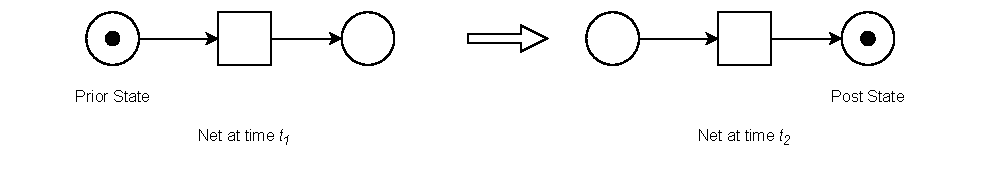
\includegraphics[width=\textwidth]{graphics/PN_Transduction.pdf}
\caption{\textbf{Transduction:
}The transducer is represented as a square node, which will fire when a condition of at least one token as input place value is satisfied, giving rise to the resulting place value.
Places are represented as circles with or without tokens (the values).}
\label{transduction}
\end{figure}

However, a pull action from the complement muscle between the cycle can generate a halting action in between.  Thus two actors can regulate each other's action without involving any other controlling agent or actor. A fine-grain halting may lead to greater coordination.  This is one model of implementing a simple haltable-action-pattern (HAP). 

Haltability, coordination of actions, emerges due to dynamic antagonism among the zones. Having established the fundamental principles of action and haltability, we now turn to the specific biological architecture that implements these principles. The SMN model proposes that cognition emerges from a particular body plan that is shared across animal life but has been largely ignored in cognitive science.
